\chapter{INTRODUCTION}
\label{ch:introduction}

% This is Chapter 1 - Introduction
% Provide an overview of your research topic, motivation, objectives, and thesis organization

\section{Introduction}

Football is widely renowned as the world’s game, yet throughout history the processes used to identify and promote talent have largely relied on subjective human judgement and limited networks of knowledge. In times where data driven solutions are being implemented in all fields to improve efficiency and performance, football is no different, and as such it has been fostering a revolution in data analysis and statistical decision making. 

This thesis aims to bring the two sides together, that is, to find efficent and cost-effective ways to bring this statistical revolution in football to all the footballers in the world. By exploring already developed technologies and pipelines and implementing them in very accessible environments we can evaluate the possibility of advancing the whole world of football players and academies, not just the richest of the rich. 

Concretely, we will not only study the already well-researched implementation of YOLOv8 models in generating football statistics from football broadcast footage, but also look to find a balance between the accuracy and performance of each model in different levels of consumer-grade computational hardware.



\section{Background and Motivation}

During recent times, the football industry has experienced massive growth driven by the increasing broadcasting revenues, sponsorship agreements and competition prizes. As a result, the clubs are more incentivized than ever to form competitive squads and optimize their performance as much as possible in order to remain competitive in a very cut-throat field. In times where the advancements in technology are making it influential for every sector, football is no different, and the market for data driven tools that can supplement every aspect of improving performance on the field is growing in parallel with the sport.

A key part of improving performance on the pitch is finding the best players. However, due to the global nature of the sport, spanning all continents, attracting passionate players of all cultural, ethnical and economic backgrounds, being picked as a talent often resorts more to opportunity and exposure rather than pure talent and ability. As such, players from wealthier backgrounds or more advanced countries benefit from that exposure, which poses a disadvantage for the others and makes a gap in the player networks for the clubs and academies. 

Another important aspect in forming great football teams is the need to objectively evaluate players. Through statistics, we can measurably evaluate the production and contribution of players on the field and therefore remove all kinds of biases that the human eye of a scout can be prone to.



\section{Problem Statement}

Implementing statistics and data analysis in football is far from a novel concept, in fact, it has already been implemented at the top level with huge success. In the early days, football statistics were generated through meticulous manual labour in data entry (Memmert and Raabe, 2018)\cite{RN01}, before progressing into data driven methodologies based on positional information and computational analysis. This progress has enabled clubs to achieve the objective and measurable structures of information that allow them to optimize their player acquisition.  

Brighton \& Hove Albion F.C., playing in the top division of English Football are one of the clubs leading this statistical revolution in modern football. The club’s Technical Director, David Weir, attributed their rise to their extensive statistical information across many leagues worldwide (Kershaw, 2025)\cite{RN02}. 

The collection of data is the most important and difficult aspect of this revolution. The wealthiest clubs such as the aforementioned Brighton F.C. make use of very advanced, and therefore, expensive pipelines (such as wearable sensors worn by players) to truly achieve the level of statistical accuracy a club at the top level truly needs in order to reliably produce results in an extremely very cut-throat environment.
However, being “the world’s game”, football spans players and clubs of all sorts of economic backgrounds, most of which are not capable of implementing the same pipelines. This is where computer vision systems offer an accessible option, as they require only video footage coupled with a capable computing device. 

That capability varies across consumers and pipelines, and constitutes the domain of our study. This thesis investigates the accuracy-speed trade-off of the three lightest YOLOv8 models by evaluating their performance on three consumer level machines each with different capabilities. This should help further users find the best performing model for their environment and specific goals.


\begin{figure}[htbp]
    \centering
    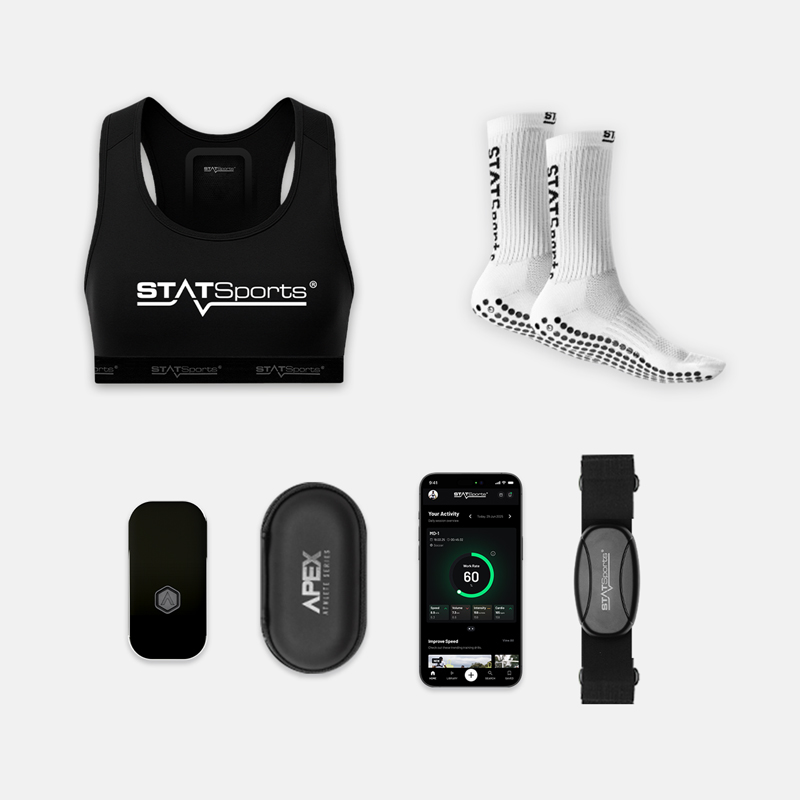
\includegraphics[width=0.85\textwidth]{figures/wearable-sensors-football.jpg}
    \caption{Wearable sensors which allow detailed player position tracking.}
    \label{fig:wearable_sensors}
\end{figure}


\section{Research Objectives}

The main goal of this thesis is to evaluate the three lightest YOLOv8 models across three different levels of hardware configurations, all accessible by average consumer such as individuals, small clubs or football academies. More specifically this seperates into:

\begin{itemize}
    \item Fine-tuning the YOLOv8n, YOLOv8s, and YOLOv8m models on the Bundesliga Data Shootout dataset under measurable and identical training conditions
    \item Evaluating the accuracy of each model using standard metrics in the field such as mAP@0.5, precision and recall.
    \item Benchmark the inference speed performance of each model across each of our selected hardware configurations by using the frames per second metric.
    \item Analyze the accuracy-speed trade-off of each model in each device, and recommend a model for each hardware level.

\end{itemize}

\section{Contributions}

The primary contributions of this thesis are summarized as follows:

\begin{enumerate}
    \item A systematic empirical comparison of YOLOv8n, YOLOv8s, and YOLOv8m trained on the Bundesliga Data Shootout dataset, providing class-level detection performance benchmarks.

    \item A hardware inference benchmark measuring the latency and throughput of each model variant across three consumer-grade hardware configurations at different price points, producing a dataset of performance results that reflects real-world deployment conditions rather than data center benchmarks.

    \item A quantitative analysis of the trade-off between detection accuracy and inference speed across the three YOLOv8 variants, identifying at which point scaling up to a larger model no longer justifies the additional computational cost on consumer-grade hardware
\end{enumerate}

\section{Thesis Organization}

This thesis is organized into five chapters, each focusing in a separate step of the research:

\textbf{Chapter 2} evaluates the current progress in the field by studying the history of object detection going to the present state-of-the-art models and the YOLO architecture family. It also provides information on prior work in football video analytics and hardware constrained video inference benchmarks.

\textbf{Chapter 3} explains in detail methodology. It describes the Bundesliga Data Shootout dataset which is used, the way it is pre-augmented, the controlled training procedure applied to each model identically and the three hardware configurations used for inference benchmarking.

\textbf{Chapter 4} presents the results of our experiment and offers the comparison of each model across different accuracy metrics and inference speed measurements on each of the three hardware configurations.

\textbf{Chapter 5} concludes the thesis through summarizing the key findings, recommending a model for each tier of hardware, discussing the limitations of our research, and pointing out directions for future research in affordable football video analytics.